\documentclass[10pt, conference]{IEEEtran}

% --- PACOTES ESSENCIAIS ---
\usepackage[utf8]{inputenc}
\usepackage[T1]{fontenc}
\usepackage[brazil]{babel}
\usepackage{amsmath, amsthm, amsfonts}
\usepackage{graphicx}
\usepackage{hyperref}
\usepackage{booktabs}
\usepackage{float}
\usepackage{listings}
\usepackage{xcolor}

% --- CONFIGURAÇÃO DO LISTINGS PARA MATLAB ---
\definecolor{commentcolor}{rgb}{0,0.6,0}
\definecolor{keywordcolor}{rgb}{0,0,1}
\definecolor{stringcolor}{rgb}{0.58,0,0.82}
\definecolor{backcolor}{rgb}{0.96,0.96,0.94}

\lstset{
    language=Matlab,
    backgroundcolor=\color{backcolor},
    commentstyle=\color{commentcolor},
    keywordstyle=\color{keywordcolor},
    stringstyle=\color{stringcolor},
    basicstyle=\ttfamily\footnotesize,
    breaklines=true,
    showstringspaces=false,
    frame=single,
    captionpos=t,
    numbers=left,
    numberstyle=\tiny\color{gray}
}

\begin{document}

\title{Relatório de Laboratório: Projeto de Filtros Digitais FIR e Processamento de Sinais no MATLAB}

\author{
  \IEEEauthorblockN{Iago Vieira Vilela, João Henrique M. P. Santos, Pedro Fernandes Aguiar, Hugo Enrico Santos Azevedo}
  \IEEEauthorblockA{UNIFEI - Campus Itabira}
}

\maketitle

\begin{abstract}
Este relatório apresenta o projeto, simulação e aplicação de Filtros Digitais com Resposta ao Impulso Finita (FIR) utilizando o software MATLAB. A primeira parte aborda o projeto de filtros passa-baixas e passa-faixa utilizando a técnica de janelamento, comparando as janelas de Hamming, Blackman e a janela ótima de Kaiser em termos de ordem e atenuação obtidas. A segunda parte foca na aplicação prática de processamento de sinais de áudio, utilizando o arquivo \texttt{fugee.wav} corrompido por ruído. Foram projetados e testados filtros FIR passa-altas e passa-faixa lineares, bem como um filtro não-linear de mediana de ordem 5. Os resultados comprovam a superioridade dos filtros não-lineares na remoção de ruídos impulsivos.
\end{abstract}

\section{Introdução Teórica}
A filtragem digital é uma operação fundamental no Processamento Digital de Sinais (PDS), cujo objetivo é modificar o conteúdo espectral de um sinal de entrada de acordo com especificações de projeto. Os filtros de resposta ao impulso finita (FIR) apresentam como principais vantagens a estabilidade inerente (por possuírem apenas zeros no plano Z) e a possibilidade de fase exatamente linear, garantindo atraso de grupo constante e evitando distorções de fase no sinal filtrado, o que é crucial em áudio de alta fidelidade.

O método de janelamento consiste em truncar a resposta ao impulso ideal $h_d[n]$ (que possui duração infinita e é não-causal) multiplicando-a por uma função de janela causal $w[n]$ de comprimento finito $M$:
\begin{equation}
h[n] = h_d[n] \cdot w[n], \quad 0 \leq n \leq M-1
\end{equation}

No domínio da frequência, isso equivale à convolução periódica entre a resposta em frequência ideal $H_d(e^{j\omega})$ e o espectro da janela $W(e^{j\omega})$. Essa operação introduz ondulações (\textit{ripples}) na banda de passagem e de corte devido aos lóbulos laterais da janela (fenômeno de Gibbs) e alarga a banda de transição devido à largura do lóbulo principal.

As principais janelas utilizadas e suas especificações típicas de atenuação mínima na banda de corte ($A_s$) e largura de transição aproximada ($\Delta f$) são apresentadas na Tabela \ref{tab:janelas_teoricas}.

\begin{table}[H]
\centering
\caption{Características das Funções de Janela}
\label{tab:janelas_teoricas}
\begin{tabular}{ccc}
\toprule
\textbf{Janela} & \textbf{Lóbulo Lateral Principal (dB)} & \textbf{Atenuação $A_s$ (dB)} \\ \midrule
Retangular & -13 & 21 \\
Hanning (Hann) & -31 & 44 \\
Hamming & -41 & 53 \\
Blackman & -57 & 74 \\ \bottomrule
\end{tabular}
\end{table}

A janela de Kaiser destaca-se como uma aproximação ótima, pois permite o controle contínuo do compromisso entre a largura do lóbulo principal e a atenuação dos lóbulos laterais por meio de um parâmetro de forma $\beta$, calculado a partir da atenuação mínima desejada na banda de corte $A_s$.

\section{Funções de Suporte}
Para viabilizar o projeto dos filtros e a plotagem correta de suas respostas em magnitude (em escala dB), foram desenvolvidas duas funções principais no MATLAB:

\begin{lstlisting}[caption={Função para resposta ao impulso ideal de um filtro passa-baixas.}]
function hd = ideal_lp(wc, M)
    alpha = (M - 1)/2;
    n = [0:(M-1)];
    m = n - alpha + eps; 
    hd = sin(wc*m)./(pi*m);
end
\end{lstlisting}

A função \texttt{ideal\_lp} calcula o sinal sinc ideal correspondente ao passa-baixas com frequência de corte $\omega_c$ e comprimento $M$, adicionando o termo infinitesimal \texttt{eps} para evitar divisão por zero no ponto de simetria $n = \alpha$.

\begin{lstlisting}[caption={Função para cálculo da resposta em frequência em escala dB.}]
function [db, mag, pha, w] = freqz_m(b, a)
    [H, w] = freqz(b, a, 1000, 'whole');
    H = (H(1:501))';
    w = (w(1:501))';
    mag = abs(H);
    db = 20*log10((mag + eps)/(max(mag)));
    pha = angle(H);
end
\end{lstlisting}

A função \texttt{freqz\_m} discretiza o espectro do filtro digital em 1000 pontos sobre o círculo unitário e extrai os primeiros 501 pontos correspondentes ao intervalo $[0, \pi]$ rad/amostra.

\section{Tarefa Prática 1.1 e 1.2: Projeto de Filtro Passa-Baixas}
As especificações exigidas para o filtro passa-baixas FIR são:
\begin{itemize}
    \item Frequência de passagem: $\omega_p = 0,2\pi$ rad/amostra.
    \item Frequência de corte da banda de rejeição: $\omega_s = 0,3\pi$ rad/amostra.
    \item Ondulação na banda de passagem: $R_p = 0,25$ dB.
    \item Atenuação mínima na banda de corte: $A_s = 50$ dB.
\end{itemize}

A largura da banda de transição é dada por $\Delta\omega = \omega_s - \omega_p = 0,1\pi$ rad/amostra, o que equivale a $\Delta f = 0,05$. A frequência de corte ideal é a média aritmética das frequências de transição: $\omega_c = 0,25\pi$.

\subsection{Projeto com Janela de Hamming (Tarefa 1.1)}
Para atingir a atenuação mínima de $50$ dB, a janela de Hanning não é adequada pois oferece apenas $44$ dB de atenuação. A janela de Hamming foi selecionada por fornecer uma atenuação típica de $53$ dB ($A_s \geq 50$ dB).

O comprimento teórico da janela é calculado por:
\begin{equation}
M = \left\lceil \frac{3,3}{\Delta f} \right\rceil = \left\lceil \frac{3,3}{0,05} \right\rceil = 66
\end{equation}

Para garantir que o filtro projetado possua ordem par ($N = M-1$), mantendo simetria de Tipo I (com atraso de grupo inteiro e sem restrições em frequências críticas), adotou-se o comprimento ímpar $M = 67$ (ordem $N = 66$). A resposta ao impulso e a magnitude em frequência do filtro projetado estão ilustradas na Fig. \ref{fig:tarefa1_1}.

\begin{figure}[H]
    \centering
    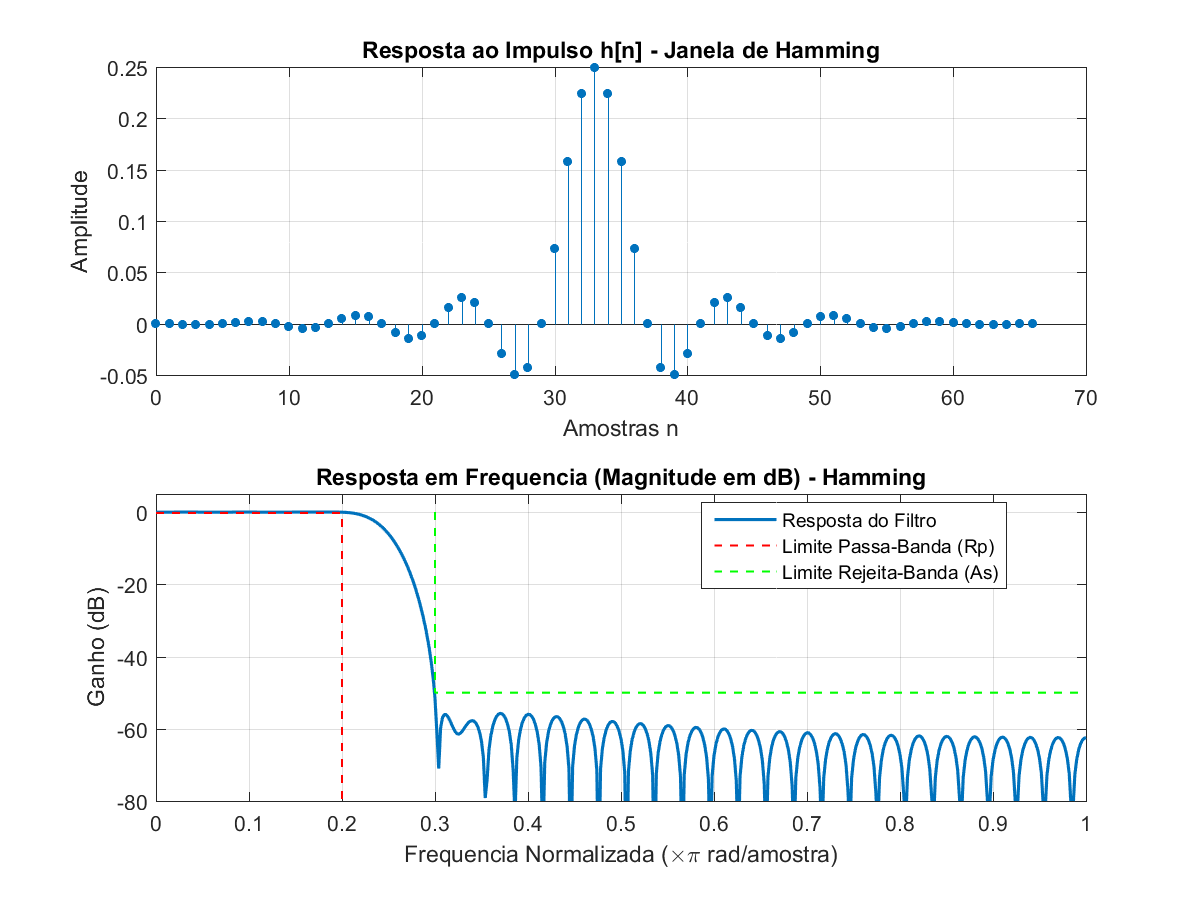
\includegraphics[width=1\linewidth]{tarefa1_1.png}
    \caption{Resposta ao impulso e magnitude em frequência do filtro passa-baixas projetado com a Janela de Hamming.}
    \label{fig:tarefa1_1}
\end{figure}

\subsection{Projeto com Janela de Kaiser (Tarefa 1.2)}
Repetiu-se o projeto utilizando a janela ótima de Kaiser. O parâmetro $\beta$ e o comprimento $M$ foram obtidos numericamente através das expressões de projeto de Kaiser. Dado que $A_s = 50$ dB, o parâmetro de forma $\beta$ foi calculado como:
\begin{equation}
\beta = 0,5842(50 - 21)^{0,4} + 0,07886(50 - 21) = 4,5335
\end{equation}

O comprimento calculado foi:
\begin{equation}
M = \left\lceil \frac{50 - 8}{2,285 \cdot (0,1\pi)} \right\rceil = \lceil 58,51 \rceil = 59
\end{equation}

Assim, o comprimento adotado foi $M = 59$ (ordem $N = 58$). A comparação direta entre os coeficientes da resposta ao impulso e a resposta em frequência dos filtros Hamming e Kaiser é apresentada na Fig. \ref{fig:tarefa1_2}.

\begin{figure}[H]
    \centering
    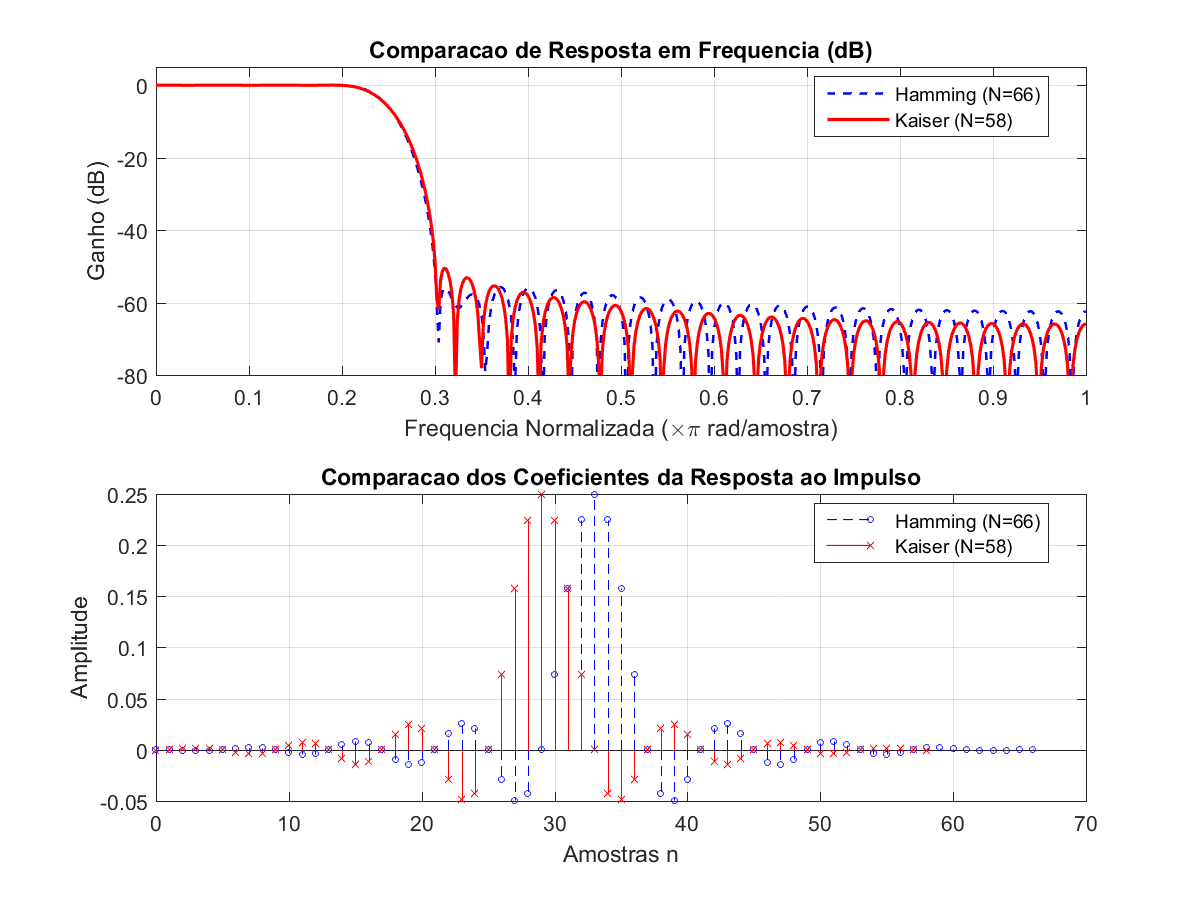
\includegraphics[width=1\linewidth]{tarefa1_2.png}
    \caption{Comparação espectral e temporal entre os filtros Hamming ($N=66$) e Kaiser ($N=58$).}
    \label{fig:tarefa1_2}
\end{figure}

O filtro projetado com a janela de Kaiser atingiu exatamente os mesmos requisitos de projeto que a janela de Hamming, exigindo uma ordem inferior ($N=58$ contra $N=66$). Isso representa uma redução de aproximadamente 12\% no custo computacional do filtro (menos multiplicações e adições por amostra).

\section{Tarefa Prática 1.3: Projeto Avançado Multibanda}
Projetou-se um filtro passa-faixa com as seguintes especificações:
\begin{itemize}
    \item Banda de corte inferior: $\omega_{1s} = 0,2\pi$ rad/amostra, $A_s = 60$ dB.
    \item Banda de passagem: de $\omega_{1p} = 0,35\pi$ a $\omega_{2p} = 0,65\pi$ rad/amostra, com $R_p = 1$ dB.
    \item Banda de corte superior: $\omega_{2s} = 0,8\pi$ rad/amostra, $A_s = 60$ dB.
\end{itemize}

A largura das duas bandas de transição é $\Delta\omega = 0,15\pi$ ($\Delta f = 0,075$). A atenuação mínima exigida nas bandas de corte é de $60$ dB.

\subsection{Projeto com Janela de Blackman}
Para satisfazer a atenuação mínima de $60$ dB, a janela de Hamming ($53$ dB) não é suficiente. Selecionou-se a janela de Blackman, que provê atenuação típica de $74$ dB. O comprimento teórico é:
\begin{equation}
M = \left\lceil \frac{5,5}{0,075} \right\rceil = 74 \implies M = 75 \text{ (Ordem } N=74\text{)}
\end{equation}

\subsection{Projeto com Janela de Kaiser}
Utilizando as equações de Kaiser com $A_s = 60$ dB:
\begin{equation}
\beta = 0,1102(60 - 8,7) = 5,6533
\end{equation}
\begin{equation}
M = \left\lceil \frac{60 - 8}{2,285 \cdot (0,15\pi)} \right\rceil = \lceil 48,29 \rceil = 49 \text{ (Ordem } N=48\text{)}
\end{equation}

A resposta ao impulso ideal foi calculada pela subtração de dois passa-baixas ideais com frequências de corte $\omega_{c1} = 0,275\pi$ e $\omega_{c2} = 0,725\pi$:
\begin{equation}
h_{d,bp}[n] = ideal\_lp(\omega_{c2}, M) - ideal\_lp(\omega_{c1}, M)
\end{equation}

A Fig. \ref{fig:tarefa1_3} ilustra a comparação das respostas em magnitude e coeficientes. A janela de Kaiser atinge a especificação com ordem $N = 48$ em comparação com a ordem $N = 74$ da Blackman, economizando 26 coeficientes (redução de 35\% em complexidade).

\begin{figure}[H]
    \centering
    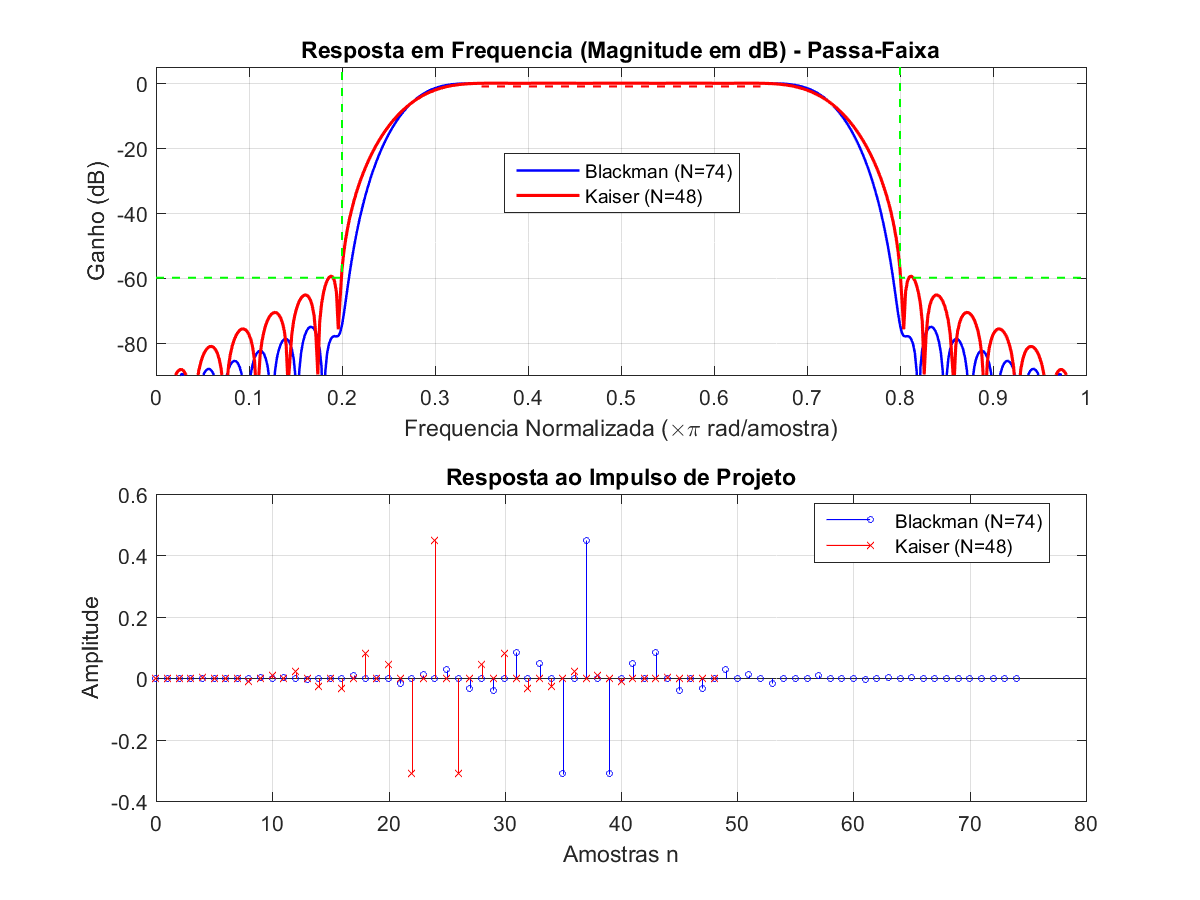
\includegraphics[width=1\linewidth]{tarefa1_3.png}
    \caption{Comparação de desempenho entre os filtros Blackman ($N=74$) e Kaiser ($N=48$) para especificações passa-faixa.}
    \label{fig:tarefa1_3}
\end{figure}

\section{Parte 3: Aplicação em Processamento de Áudio}
O sinal \texttt{fugee.wav} foi importado no MATLAB. Ele possui taxa de amostragem $F_s = 8$ kHz (Nyquist em $4$ kHz), canal único (mono) e duração aproximada de $299,11$ segundos.

\subsection{Análise do Sinal Corrompido}
O sinal temporal e o espectro de magnitude original são mostrados na Fig. \ref{fig:audio_orig}. A análise no domínio do tempo revela a presença de pulsos de altíssima amplitude e curtíssima duração (picos verticais estreitos), o que indica que o áudio está corrompido por \textbf{ruído impulsivo}. Fisicamente, esse tipo de ruído se traduz por estalos e estalos audíveis (tipo \textit{clicks}). No domínio da frequência, o espectro exibe um elevado patamar de ruído de fundo plano e distribuído, característico de impulsos aproximados pela função delta de Dirac.

\begin{figure}[H]
    \centering
    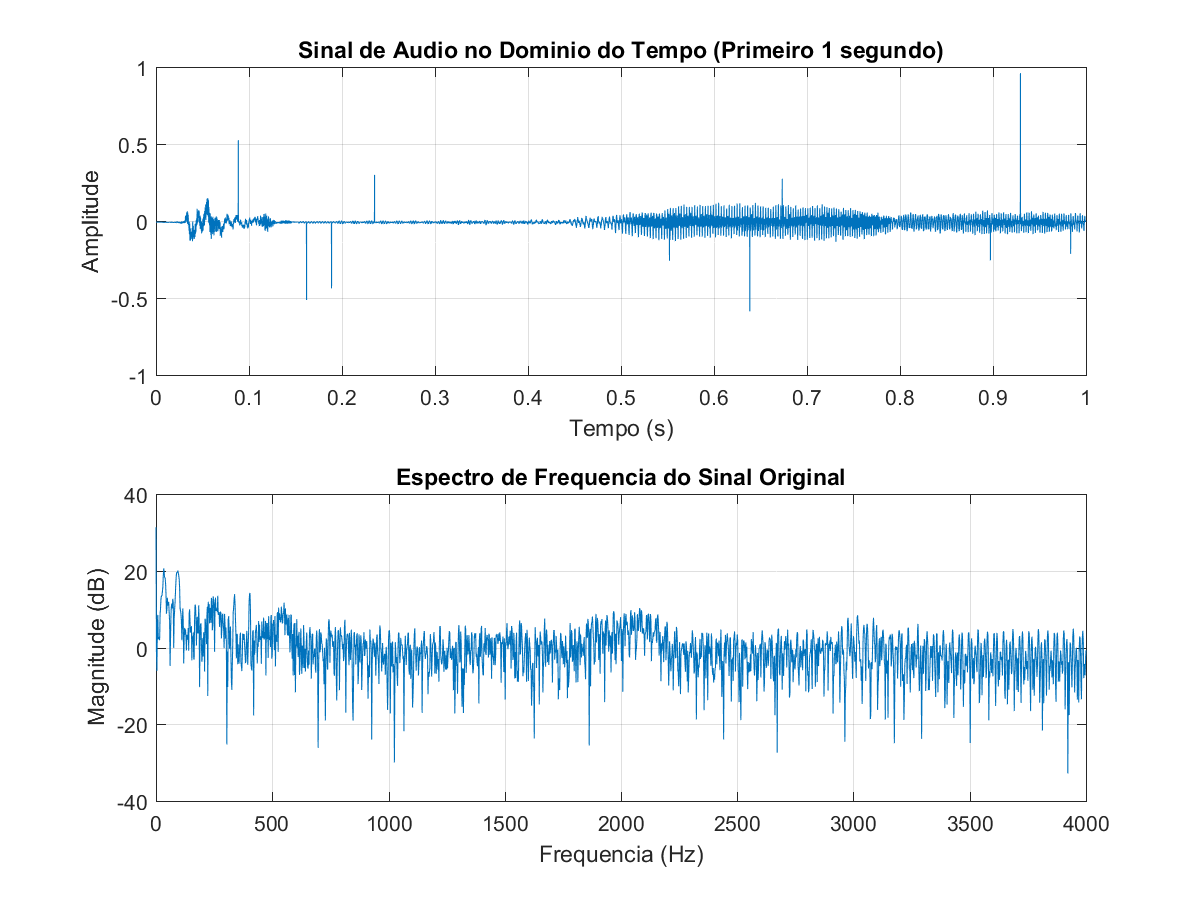
\includegraphics[width=1\linewidth]{audio_original.png}
    \caption{Forma de onda e espectro de magnitude original do sinal \texttt{fugee.wav}.}
    \label{fig:audio_orig}
\end{figure}

\subsection{Filtragem Linear (FIR)}
Foram implementados dois filtros lineares para tentar limpar o sinal de ruído:
\begin{enumerate}
    \item \textbf{Cenário 1 (Passa-Altas):} Filtro passa-altas FIR de ordem 34, frequência de corte normalizada de $0,45\pi$ rad/amostra (equivalente a $1800$ Hz), utilizando janela de Chebyshev com atenuação de 30 dB.
    \item \textbf{Cenário 2 (Passa-Faixa):} Filtro passa-faixa FIR de ordem 48, com banda passante entre $0,65\pi$ e $0,75\pi$ rad/amostra (equivalente a $[2600\text{ Hz}, 3000\text{ Hz}]$), utilizando janela padrão de Hamming.
\end{enumerate}

O efeito da filtragem passa-faixa no sinal de voz é severo. A banda passante estreita remove quase todo o conteúdo espectral da voz (especialmente as baixas frequências que contêm a energia e formantes da fala). Como resultado, a voz torna-se abafada, altamente metálica e a inteligibilidade é significativamente prejudicada. Adicionalmente, os filtros lineares espalham os transientes do ruído impulsivo no tempo devido à convolução com a resposta ao impulso do filtro, atenuando a amplitude dos picos mas prolongando os cliques sob a forma de oscilações (efeito de \textit{ringing}).

\subsection{Filtragem Não-Linear (Mediana)}
Aplicou-se um filtro não-linear de mediana com janela de dimensão 5 (\texttt{medfilt1(x, 5)}). 

A Fig. \ref{fig:audio_comp} apresenta o espectro original comparado com as saídas obtidas por cada um dos filtros testados.

\begin{figure}[H]
    \centering
    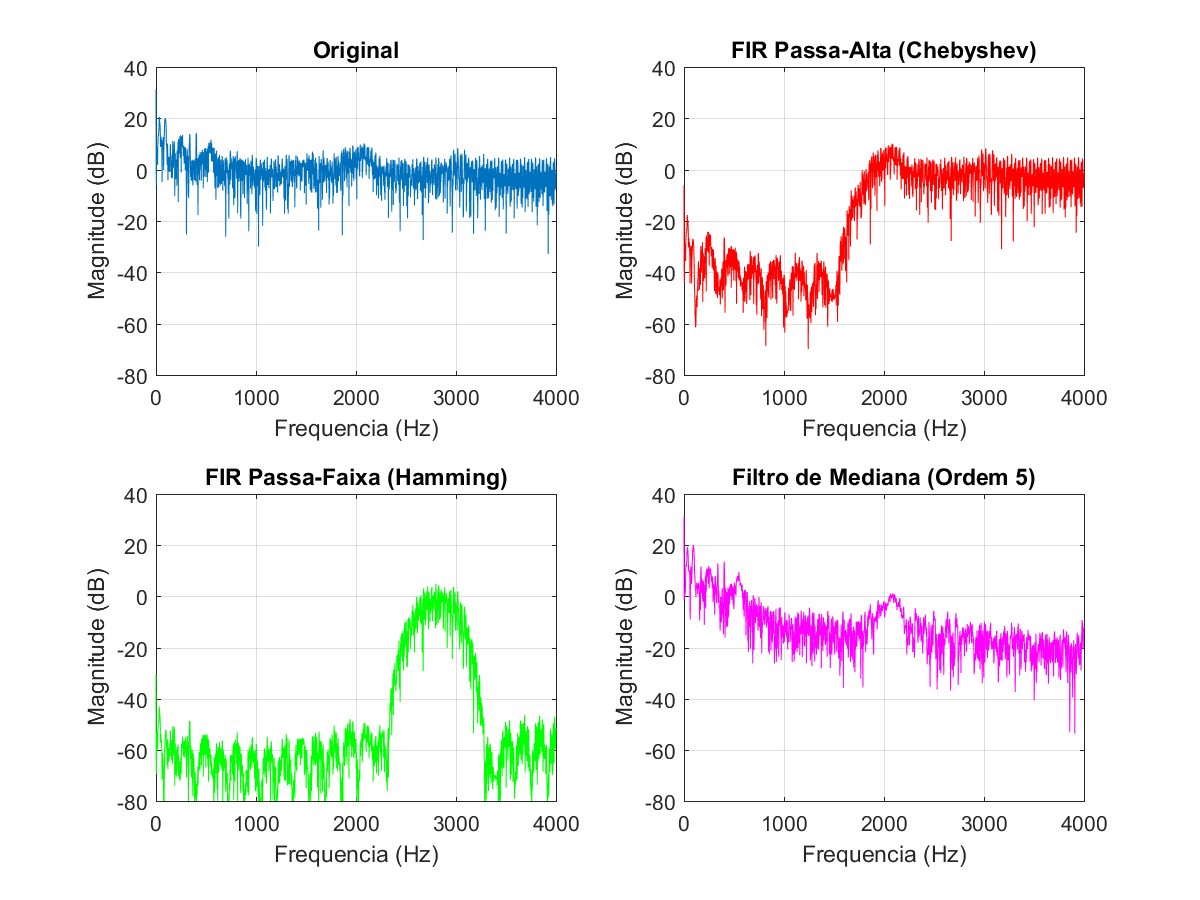
\includegraphics[width=1\linewidth]{audio_comparacao_espectros.png}
    \caption{Comparação dos espectros de frequência obtidos após aplicação dos filtros linear (FIR) e não-linear (Mediana).}
    \label{fig:audio_comp}
\end{figure}

O filtro de mediana foi \textbf{muito superior} aos filtros lineares FIR. Sendo o ruído impulsivo composto por amostras discrepantes (outliers) isoladas e de curta duração, o cálculo da mediana em uma janela local de 5 amostras substitui com sucesso o valor ruidoso pelo valor representativo dos seus vizinhos de baixa amplitude. Como evidenciado na Fig. \ref{fig:audio_comp} (canto inferior direito), o filtro de mediana abaixou consideravelmente o patamar de ruído em todo o espectro, preservando a forma e a potência espectral do sinal de voz fundamental, obtendo um áudio limpo de estalos sem perdas de qualidade perceptíveis.

\section{Conclusão}
Este experimento demonstrou de forma prática a eficácia das técnicas de projeto de filtros FIR por janelamento no MATLAB. Constatou-se que a janela de Kaiser oferece projetos muito mais otimizados em termos de ordem em relação às janelas fixas clássicas (como Hamming e Blackman), reduzindo de forma expressiva o custo computacional para uma mesma especificação. Adicionalmente, a análise do processamento de áudio evidenciou os limites dos filtros lineares de frequência na presença de ruído impulsivo e demonstrou a ampla eficiência dos filtros não-lineares baseados em ordenação (mediana) para a restauração de sinais corrompidos por transientes rápidos.

\begin{thebibliography}{1}
\bibitem{roteiro}
Equipe Docente, \emph{Projeto de Filtros Digitais FIR e IIR no MATLAB}, Roteiro de Laboratório de Processamento Digital de Sinais (PDS), 2026.
\bibitem{proakis}
J. G. Proakis, D. G. Manolakis, \emph{Digital Signal Processing: Principles, Algorithms, and Applications}, 4th ed., Prentice Hall, 2007.
\end{thebibliography}

\end{document}
